\section{Parallel System}
\label{sec:mod:parallel}

The parallel compressor system, shown in Figure~\ref{fig:mod:parallel} consists of two compressors whose discharge tanks both feed into a common tank, which has a separate discharge valve and a downstream atmospheric pressure boundary condition.
For simplicity, the two compressors are assumed to have identical parameters and behavior, and the discharge valve of the common tank is assumed to have the same characteristic as the discharge valves of the compressors.

\begin{figure}[]
  \centering
  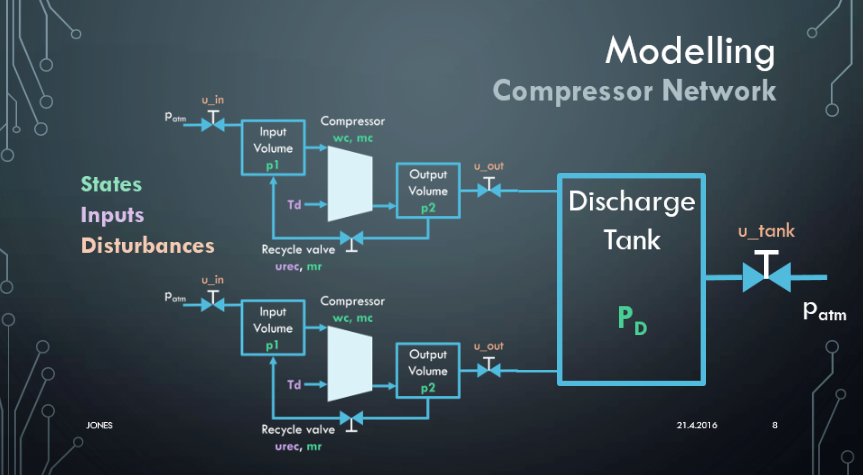
\includegraphics[width=\linewidth]{modelling/parallel_diagram.png}
  \caption{Diagram of parallel compressor system}
  \label{fig:mod:parallel}
\end{figure}


The model used has 11 states in total: 5 states for each compressor, as described above, and another state for the pressure in the common tank. It's dynamics are given by:

\begin{equation}
  \dt{}\begin{bmatrix}
    \vec{x_1}\\
    \vec{x_2}\\
    p_\text{t}
  \end{bmatrix}
  =
  \begin{bmatrix}
    \vec{f_1}\\
    \vec{f_2}\\
    \frac{a^2}{V_\text{t}}\left(q_{\text{d,1}}+q_{\text{d,2}}-q_{\text{d,t}}\right)
  \end{bmatrix},
\end{equation}

\begin{equation}
  \begin{split}
    q_{\text{d,1}} & = q_{\text{d,1}}(\vec{\varepsilon_1},\ u_{\text{out},1},\ p_{\text{t}},\ p_{\text{d,1}})\\
    q_{\text{d,2}} & = q_{\text{d,2}}(\vec{\varepsilon_2},\ u_{\text{\text{out}},2},\ p_{\text{t}},\ p_{\text{d,2}})\\
    q_{\text{d,t}} & = q_{\text{d,t}}(\vec{\rho},\ u_{\text{t}},\ p_\text{t},\ p_{\text{out}})
  \end{split}
\end{equation}

where:

\begin{itemize}
  \item $\vec{x}$ and $\vec{f}$ are the states and derivatives of a single compressor, defined in \eqref{eq:mod:single_comp_states};
  \item $p_\text{t}$ and $V_\text{t}$ are the pressure and the volume of the common tank, respectively; 
  \item $q_{\text{d,t}}$ is the mass flow across the common tank discharge valve;
  \item $\vec{\rho}$ contains the coefficients mapping the mass flow through the common tank discharge valve to the pressure differential across the valve;
  \item $u_\text{t}$ is the discharge valve opening of the common tank; and
  \item the subscripts 1 and 2 refer to values for the first and second compressor, respectively.
\end{itemize}

The inputs to the system are thus the suction, discharge and recycle valve positions for each compressor, the torque input for each compressor, and the common tank discharge valve position.
The discharge valves linking each compressor to the common tank ($u_{\text{out},1}$ and $u_{\text{out},2}$) are, however, kept in a fully open position in order to reduce the pressure losses in the system.

